
As a starting example, we consider analysis of PK and PD data from a
single patient using a PKPD model described in terms of a nonlinear ODE
system that requires the use of a numerical solver.
The patient receives multiple doses at regular time intervals and the drug plasma concentration is recorded over time.

\subsection{Nonlinear pharmacokinetic / pharmacodynamic model} 
For the last example, let us go back to the single patient
two-compartment model and append it with a PD
model. Specifically, we examine the
Friberg-Karlsson semi-mechanistic model for drug-induced
myelosuppression \cite{3181,2364,2518,3187,3188,3537} with the goal to model the
relation between neutrophil counts and drug exposure.
It describes a delayed feedback mechanism that keeps the absolute neutrophil count (ANC) at the
baseline ($\text{Circ}_0$) in a circulatory compartment ($y_{\text{circ}}$), as well as the drug
effect that perturbs this meachanism. The delay between
proliferative cells ($y_{\text{prol}}$) and $y_{\text{circ}}$ is modeled by three
transit compartments with mean transit time
\begin{equation}
  \text{MTT} = (3 + 1)/k_{\text{tr}}
\end{equation}
where $k_{\text{tr}}$ is the transit rate constant.
\begin{figure}
  \begin{center}
  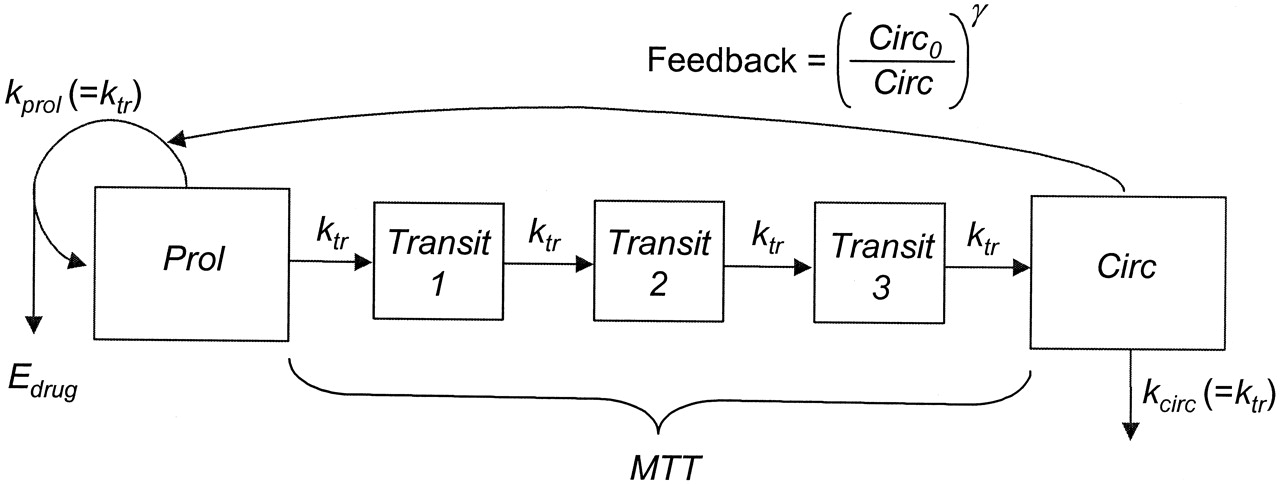
\includegraphics[width=5in]{../figures/neutrophilModel.jpg}
  \caption{Friberg-Karlsson semi-mechanistic Model.}
  \label{fig:fk_model}
  \end{center}
\end{figure}

The PD model can be summarized as
\begin{align*}
  \log(\text{ANC})& \sim \text{Normal}(\log(y_{\text{circ}}), \sigma^2_{\text{ANC}}),  \\
  y_{\text{circ}}& = f_{\text{FK}}(\text{MTT}, \text{Circ}_{0}, \alpha, \gamma, c),
  % (\text{MTT}, \text{Circ}_{0}, \alpha, \gamma, k_{\text{tr}})& = (125, 5.0, 3 \times 10^{-4}, 0.17) \\
  % \sigma^2_{\text{ANC}}& = 0.001
\end{align*}
where $c=y_{\text{cent}}/V_{\text{cent}}$ is the drug concentration calculated from the PK model, and function $f_{\text{FK}}$ represents solving  the following
nonlinear ODE for $y_{\text{circ}}$ 
\begin{subequations}\label{eq:FK}
\begin{align}
  \frac{dy_\mathrm{prol}}{dt} &= k_\mathrm{prol} y_\mathrm{prol} (1 - E_\mathrm{drug})\left(\frac{\text{Circ}_0}{y_\mathrm{circ}}\right)^\gamma - k_\mathrm{tr}y_\mathrm{prol}, \\
  \frac{dy_\mathrm{trans1}}{dt} &= k_\mathrm{tr} y_\mathrm{prol} - k_\mathrm{tr} y_\mathrm{trans1}, \\
  \frac{dy_\mathrm{trans2}}{dt} &= k_\mathrm{tr} y_\mathrm{trans1} - k_\mathrm{tr} y_\mathrm{trans2},  \\
  \frac{dy_\mathrm{trans3}}{dt} &= k_\mathrm{tr} y_\mathrm{trans2} - k_\mathrm{tr} y_\mathrm{trans3},  \\
  \frac{dy_\mathrm{circ}}{dt} &= k_\mathrm{tr} y_\mathrm{trans3} - k_\mathrm{tr} y_\mathrm{circ},
\end{align}
\end{subequations}
We use $E_{\text{drug}} = \alpha c$ to model the linear effect of drug
concentration in central compartment that reduces the proliferation rate or induces cell loss. The entire ODE system is formed by coupling equation \eqref{eq:twocpt}
and \eqref{eq:FK}.
The following \texttt{parameters} block summarizes the unknown parameters this model
\lstinputlisting[firstline=87,lastline=102]{../../Script/neutropenia-single-patient/neutropeniaSinglePatient1.stan}

Unlike in Section \ref{sec:twocpt}, here to solve the nonlinear system we must
utilize one of the numerical solvers in Torsten.

\subsubsection{Numerical solution of ODE}
To solve an ODE numerically in Stan we first need to define
its right-hand-side in the \texttt{functions} block, a block in which
we put all the user-supplied functions.
\lstinputlisting[firstline=1,lastline=38]{../../Script/neutropenia-single-patient/neutropeniaSinglePatient1.stan}
One can see that the above function is almost literal translation of
Eq. \eqref{eq:twocpt} and \eqref{eq:FK}, in that the first three
components of \texttt{dydt} describes the PK while the rest the
PD.

We omit most items in the \texttt{data} block but bring reader's attention to a
few items. It often helps to keep an index array that points to the
observations in the ODE solutions, such as
\lstinputlisting[firstline=50,lastline=51]{../../Script/neutropenia-single-patient/neutropeniaSinglePatient1.stan}
which are the indices to the the drug concentration and neutrophils
count observations, respectively. Though Stan/Torsten provides
default values, we highly recommend that the user define the ODE
solver control parameters in the \texttt{data} block
\lstinputlisting[firstline=70,lastline=72]{../../Script/neutropenia-single-patient/neutropeniaSinglePatient1.stan}
and judiciously choose these control parameters
\begin{itemize}
\item \texttt{rtol}: relative tolerance to determine solution convergence,
\item \texttt{atol}: absolute tolerance to determine solution convergence,
\item \texttt{max\_num\_step}: maximum allowed steps.
\end{itemize}
In particular, user should make problem-dependent decision on \texttt{rtol} and \texttt{atol},
according to estimated scale of the unknowns, so that the error would
not affect inference on statistical variance of quantities that enter
the Stan model. For example, when an unknown can be neglected below
certain threshold without affecting the rest of the dynamic system,
setting \texttt{atol} greater than that threshold will avoid spurious and
error--prone computation. For more details, see \cite[Chapter 13]{Stan_users_guide:2021}
and \cite[Section 3.7.5]{Torsten:2021} and reference therein.

In \texttt{transformed data} block, we define fixed event specification
arguments such as \texttt{rate}, \texttt{ii}, etc, that are not
effective in this model. In fact here we also provide bioavailabity fraction \texttt{F} and dosing lag
time \texttt{tLag}, despite the fact that they are defined with default values
therefore can be omitted.
\lstinputlisting[firstline=75,lastline=85]{../../Script/neutropenia-single-patient/neutropeniaSinglePatient1.stan}

Now we are ready to solve the ODEs. Similar to Stan, Torsten provides
a few numerical solvers and in this
example we use the Runge-Kutta solver
\texttt{pmx\_solve\_rk45}\cite[Section 3.4]{Torsten:2021}. This
is done in the \texttt{transformed parameters} block.

\lstinputlisting[firstline=104,lastline=121]{../../Script/neutropenia-single-patient/neutropeniaSinglePatient1.stan}

One can see that \texttt{pmx\_solve\_rk45}
requires a user-defined ODE function as the first argument (similar to
how one solve an ODE using Stan function
\texttt{ode\_rk45}). In Stan functions like this are refered as
\emph{high--order functions} \cite[Chapter 9]{Stan:2021}.

\subsubsection{Solve PKPD model as coupled ODE system}
The approach in the last section applies to all the models that involve
ODE solutions, but we will not use it here. An acute
observer may have noticed the PKPD model here exhibits a particular
\emph{one-way coupling} structure.
That is, the PK (Eq. \eqref{eq:twocpt})
and PD (Eq. \eqref{eq:FK}) are
coupled through the proliferation cell count
$y_{\text{prol}}$ and $E_{\text{drug}}$ and the PK 
can be solved independently from the PD. This is what motivates Torsten's coupled solvers,
which analytically solves PK before
passing the PK solution to the PD and seeks its numerical
solution. Since the dimension of the numerical ODE solution is reduced, in general this coupled strategy is more efficient than
the last section's approach of numerically solving a full ODE system.
To see it in action, let us apply the
coupled solver \texttt{pmx\_solve\_twocpt\_rk45} \cite[Section 3.5]{Torsten:2021} to the same model. We need only make two changes. First, we
modify the ODE function to reflect that only the PD states are to be solved.
\lstinputlisting[firstline=1,lastline=30]{../../Script/neutropenia-single-patient/neutropeniaSinglePatientMix1.stan}

Note that here we pass in PK and PD states as separate arguments $y$
and $y_{\text{PK}}$, and the function describes the ODE for $y$, while
$y_{\text{PK}}$ will be solved internally using analytical solution,
so user do not need to explicitly call \texttt{pmx\_solve\_twocpt}.

Then we can simply replace \texttt{pmx\_solve\_rk45} with
\texttt{pmx\_solve\_twocpt\_rk45} call.
\lstinputlisting[firstline=108,lastline=108]{../../Script/neutropenia-single-patient/neutropeniaSinglePatientMix1.stan}

The \texttt{model} block is similar to that in Section \ref{sec:twocpt}.
\lstinputlisting[firstline=117,lastline=133]{../../Script/neutropenia-single-patient/neutropeniaSinglePatientMix1.stan}

\subsubsection{Posterior predictive checks}
We hope by now reader has developed the habit of performing
PPC on every model. Since we have both PK (drug
concentration) and PD (neutrophil count) observations, the PPC should
be conducted on both.
\lstinputlisting[firstline=135,lastline=147]{../../Script/neutropenia-single-patient/neutropeniaSinglePatientMix1.stan}

To add flexibility, \texttt{cmdstanr} packages provides a function
\texttt{generate\_quantities} so we can actually run the above code
\emph{after} the fitting run is completed. With
Stan model variable \texttt{mod} that contains the above \texttt{generated quantities}
block and fitting results \texttt{fit}, as in Section \ref{sec:call_stan_from_R},
we can do
\begin{lstlisting}[language=R, numbers=none]
fit.gq <- mod$generate_quantities(fit)
\end{lstlisting}
and use the results for PPC.
Even better, for such a routine operation in Bayesian data analysis, package \texttt{bayesplot}
provides numerous plotting functions.
\begin{lstlisting}[language=R, numbers=none]
c.rep <- fit.gq$draws(variables = c("cObsPred")) %>% as_draws_df() %>% as.matrix()
c.rep <- c.rep[ , data$iObsPK]  # use iObsPK from data to extract PK predictions corresponding to observation time

neut.rep <- fit.gq$draws(variables = c("neutObsPred")) %>% as_draws_df() %>% as.matrix()
neut.rep <- neut.rep[ , data$iObsPD]  # use iObsPD from data to extract PD predictions corresponding to observation time

c.obs <- data$cObs  # PK observations
neut.obs <- data$neutObs # PD observations

# PPC(PK): drug concentration
ppc.pk <- bayesplot::ppc_ribbon(y = c.obs, yrep = c.rep, x = data$time[data$iObsPK]) +
    scale_x_continuous(name="time (h)") +
    scale_y_continuous(name="drug plasma concentration (ng/mL)") + theme(axis.title=element_text(size=20),axis.text=element_text(size=20),legend.text=element_text(size=20))

# PPC(PD): neutrophil count
ppc.pd <- bayesplot::ppc_ribbon(y = neut.obs, yrep = neut.rep, x = data$time[data$iObsPD]) +
    scale_x_continuous(name="time (h)") +
    scale_y_continuous(name="Neutrophil counts") + theme(axis.title=element_text(size=20),axis.text=element_text(size=20),legend.text=element_text(size=20))
\end{lstlisting}

The code generates Figure \ref{fig:neutro_ppc_1} and \ref{fig:neutro_ppc_2}.
\begin{figure}
  \begin{subfigure}[b]{0.45\textwidth}
    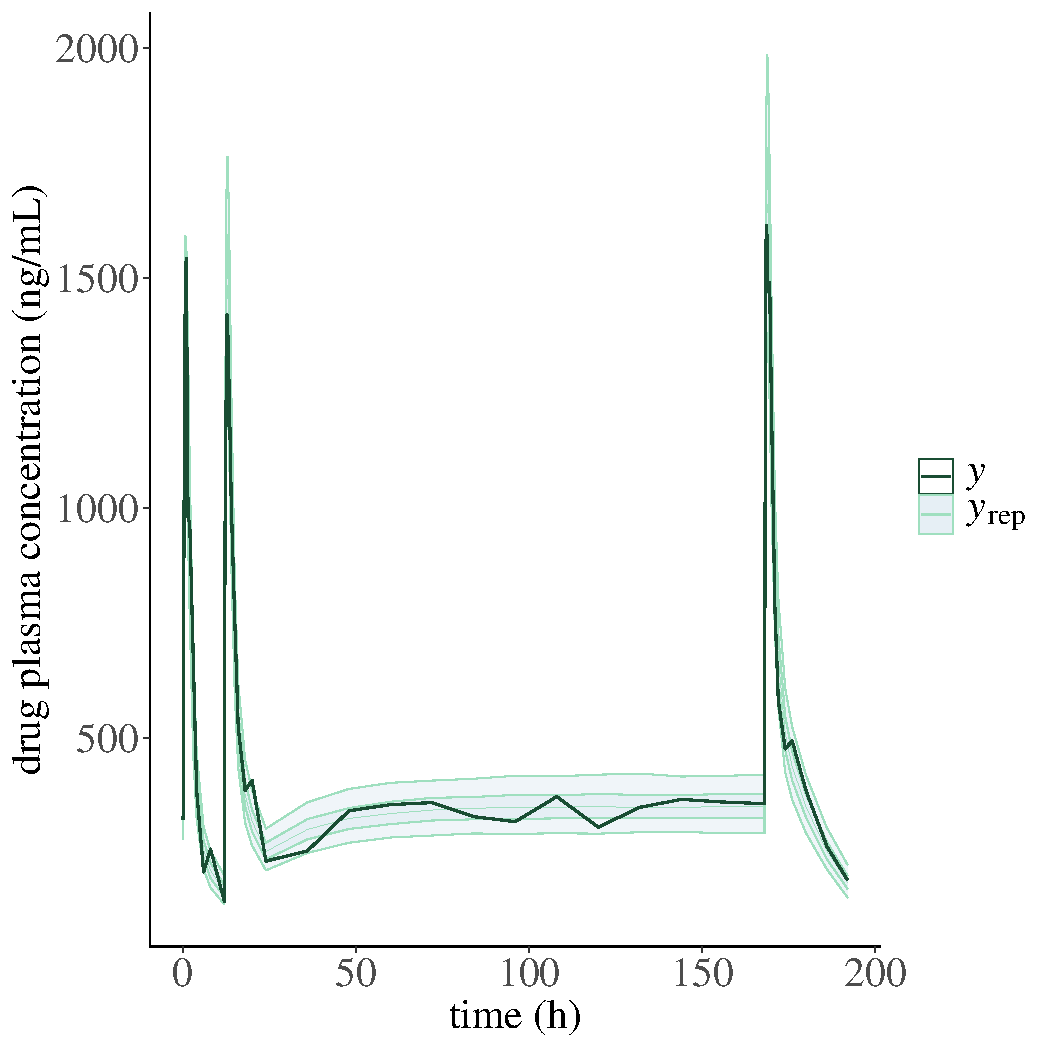
\includegraphics[width=\textwidth]{../figures/neutrophil_ppc_pk.pdf}
    \caption{PK: drug concentration}
    \label{fig:neutro_ppc_1}
  \end{subfigure}
  \qquad
  \begin{subfigure}[b]{0.45\textwidth}
    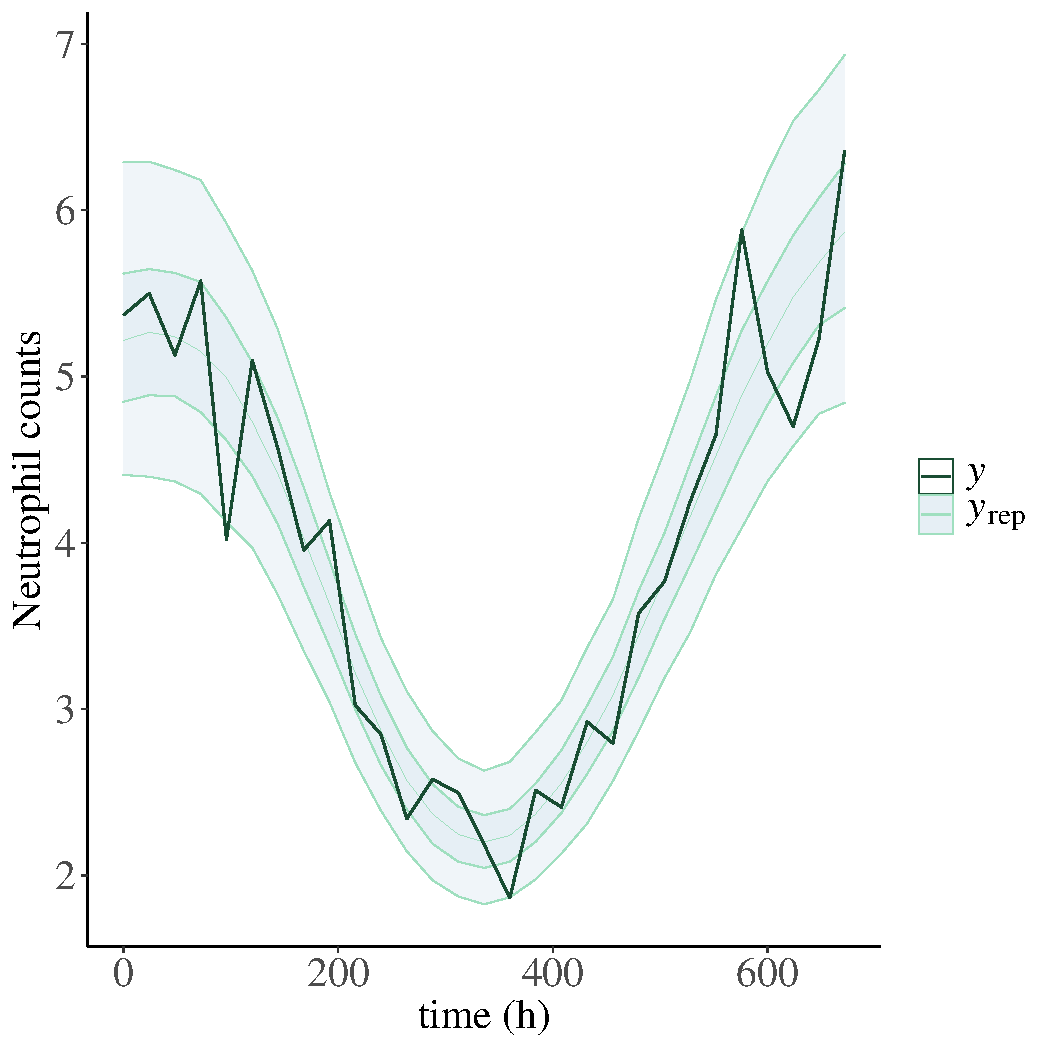
\includegraphics[width=\textwidth]{../figures/neutrophil_ppc_pd.pdf}
    \caption{PD: neutrophil count}
    \label{fig:neutro_ppc_2}
  \end{subfigure}
  \caption{Posterior predictive checks for the PKPD model}
\end{figure}
